\documentclass[conference]{IEEEtran}
\IEEEoverridecommandlockouts
% The preceding line is only needed to identify funding in the first footnote. If that is unneeded, please comment it out.
\usepackage{cite}
\usepackage{listings}
\usepackage{amsmath,amssymb,amsfonts}
\usepackage{algorithmic}
\usepackage{graphicx}
\usepackage{subcaption}
\usepackage{textcomp}
\usepackage{xcolor}
\usepackage{enumitem}
\usepackage{tabularx}
\usepackage{float}
\def\BibTeX{{\rm B\kern-.05em{\sc i\kern-.025em b}\kern-.08em
    T\kern-.1667em\lower.7ex\hbox{E}\kern-.125emX}}
\begin{document}

\title{Introduction to Computer Vision Assignment 3\\
}

\author{\IEEEauthorblockN{Lam Nguyen - 500838417}
\IEEEauthorblockA{\textit{Toronto Metropolitan University} \\
lam.nguyen@ryerson.ca}
}
\maketitle

\section{Introduction}

This assignment introduces the basic concepts for 2D projective geometry including homogeneous coordinates, conics and dual conics. In addition, the code as well as principle for robust data fitting with outliers will be investigated.

\section{Part 1}

\subsection{Problem 1}

1. Given two lines as following: 

\[ l: 0.5x + y - 2 = 0 \]
\[ l{'}: 3x + 6y - 5 = 0 \]

The intersection of two lines \(l\) and \(l{'}\) is the point \(x = l\times l{'}\)

\[ x = l\times l{'} = \begin{vmatrix}
i & j & k\\
0.5 & 1 & -2\\
3 & 6 & -5
\end{vmatrix} = \begin{pmatrix} 7\\-3.5\\0 \end{pmatrix} \]

According to the obtained result, the two lines are parallel or intersect at "infinity".

2. The general homogeneous form of an ideal point is the set for which the third homogeneous term is equal to \(0\), with \(x_1\) and \(x_2\) representing the general first and second terms of the vector:

\[ x_{ideal} = \begin{pmatrix} x_1\\x_2\\0 \end{pmatrix} \]

The general homogeneous form of the line at infinity has the first and second homogeneous terms set to \(0\), and the third homogeneous term is \(1\):

\[ l_{\infty} = \begin{pmatrix} 0\\0\\1 \end{pmatrix} \]

The point \(x\) lies on the line \(l\) if and only if the dot product of \(x\) with \(l\) is equal to \(0\). Applying this theorem to verify that the ideal point is on the line at infinity:

\[ x_{ideal}^\mathrm{T}l_{\infty} = 
\begin{pmatrix}
x_1 & x_2 & 0
\end{pmatrix}\begin{pmatrix} 0\\0\\1 \end{pmatrix} 
= 0 \]

3. The equation of a conic in inhomogeneous coordinates is

\[ ax^2 + bxy + cy^2 + dx + ey + f = 0 \]

Homogenize the above equation by the replacement \(x \mapsto x_1/x_3\), \(y \mapsto x_2/x_3\) gives

\[ a\frac{x_1^2}{x_3^2} + b\frac{x_1x_2}{x_3^2} + c\frac{x_2^2}{x_3^2} + 
d\frac{x_1}{x_3} + e\frac{x_2}{x_3} + f = 0 \]

Simplify the equation to obtain the conic in homogeneous coordinates

\[ ax_1^2 + bx_1x_2 + cx_2^2 + dx_1x_3 + ex_2x_3 + fx_3^2 = 0 \]

The equation of a conic in matrix form is 

\[ \mathrm{x}^\mathrm{T}\mathrm{C}\mathrm{x} = 0 \]

where 

\[ \mathrm{C} = \begin{bmatrix}
a & b/2 & d/2\\
b/2 & c & e/2\\
d/2 & e/2 & f
\end{bmatrix} \]

\clearpage

\subsection{Problem 2}

1. A general 2D point transformation  requires 9 multiplies and 6 adds

\[ \begin{pmatrix} x{'}\\y{'}\\z{'} \end{pmatrix} = 
\begin{bmatrix}
a & b & c\\
d & e & f\\
g & h & i
\end{bmatrix}\begin{pmatrix} x\\y\\z \end{pmatrix}
 \]
 
 \[ \begin{pmatrix} x{'}\\y{'}\\z{'} \end{pmatrix} = 
\begin{bmatrix}
ax + by + cz\\
dx + ey + fz\\
gx + hy + iz
\end{bmatrix}
 \]
 
For an ideal point, the homogeneous term \( z \) is set to zero
 
 \[ \begin{pmatrix} x{'}\\y{'}\\z{'} \end{pmatrix} = 
\begin{bmatrix}
a & b & c\\
d & e & f\\
g & h & i
\end{bmatrix}\begin{pmatrix} x\\y\\0 \end{pmatrix} =
\begin{bmatrix}
ax + by \\
dx + ey \\
gx + hy 
\end{bmatrix}
 \]
 
 Therefore under a general 2D transformation, an ideal point is mapped to a finite point. 

2. Given point transformation \(\mathrm{x}_{i}{'} = \mathrm{H}\mathrm{x}_i\), then the inverted point transformation is 

\[\mathrm{x}_i = \mathrm{H}^{-1}\mathrm{x}_{i}{'}\]

The line transformation obtained by applying inverted point transformation is 

\[l^\mathrm{T}\mathrm{x}_i = l^\mathrm{T}\mathrm{H}^{-1}\mathrm{x}_{i}{'} =
{(\mathrm{H}^\mathrm{-T}l)}^\mathrm{T}\mathrm{x}_{i}{'} \]

Therefore, the result of the line transformation is 

\[l{'} = \mathrm{H}^\mathrm{-T}l \]

Similarly, the conic's matrix transforms 

\[ \mathrm{x}_i^\mathrm{T}\mathrm{C}\mathrm{x}_i =  (\mathrm{H}^{-1}\mathrm{x}_{i}{'})^\mathrm{T}\mathrm{C}(\mathrm{H}^{-1}\mathrm{x}_{i}{'}) =
\mathrm{x}_{i}{'}^\mathrm{T}(\mathrm{H}^\mathrm{-T}\mathrm{C}\mathrm{H}^{-1})\mathrm{x}_{i}{'} \]

\[ \therefore \mathrm{C}{'} = \mathrm{H}^\mathrm{-T}\mathrm{C}\mathrm{H}^{-1} \]

\clearpage
\subsection{Problem 3}

1. A projective transformation is given by a general non-singular linear transformation of homogeneous coordinates, represented as

\[ \begin{pmatrix} x_1{'}\\x_2{'}\\x_3{'} \end{pmatrix} = 
\begin{bmatrix}
h_{11} & h_{12} & h_{13}\\
h_{21} & h_{22} & h_{23}\\
h_{31} & h_{32} & h_{33}
\end{bmatrix}\begin{pmatrix} x_1\\x_2\\x_3 \end{pmatrix}
 \]
 
 or in the block form
 
 \[ \mathrm{x}{'} = \mathrm{H}_\mathrm{P}\mathrm{x} = 
 \begin{bmatrix}
\mathrm{A}& \mathrm{t} \\
\mathrm{v}^\mathrm{T} & \upsilon
\end{bmatrix}\mathrm{x}
 \]

A projective transformation has eight degrees of freedom and can be computed from four point correspondences.

Invariant properties of projective transformation: 

\begin{description}[font=$\bullet$~\normalfont\scshape\color{red!50!black}]
  \item Concurrency
  \item Collinearity
  \item Order of contact
  \item Cross ratio
\end{description}

An affine transformation (or affinity) is a non-singularlineartransformation followed
by a translation, given by

\[ \begin{pmatrix} x{'}\\y{'}\\1 \end{pmatrix} = 
\begin{bmatrix}
a_{11} & a_{12} & t_{x}\\
a_{21} & a_{22} & t_{y}\\
0 & 0 & 1
\end{bmatrix}\begin{pmatrix} x\\y\\1 \end{pmatrix}
 \]
 
 or in the block form
 
 \[ \mathrm{x}{'} = \mathrm{H}_\mathrm{A}\mathrm{x} = 
 \begin{bmatrix}
\mathrm{A}& \mathrm{t} \\
0^\mathrm{T} & 1
\end{bmatrix}\mathrm{x}
 \]
 
A planar affinity has six degrees of freedom and can be computed from three point correspondences.

Invariant properties of affine transformation: 

\begin{description}[font=$\bullet$~\normalfont\scshape\color{red!50!black}]
  \item Parallelism
  \item Ratio of areas
  \item Ratio of length on collinear or parallel lines
  \item Linear combinations of vectors
  \item The line at infinity, \( l_{\infty} \)
\end{description}

A similarity transformation (or similarity) is an isometry composed with an isotropicscaling. With no reflection, the similarity has matrix representation

\[ \begin{pmatrix} x{'}\\y{'}\\1 \end{pmatrix} = 
\begin{bmatrix}
scos\theta & -ssin\theta & t_{x}\\
ssin\theta & -scos\theta & t_{y}\\
0 & 0 & 1
\end{bmatrix}\begin{pmatrix} x\\y\\1 \end{pmatrix}
 \]
 
 or in the block form
 
 \[ \mathrm{x}{'} = \mathrm{H}_\mathrm{S}\mathrm{x} = 
 \begin{bmatrix}
s\mathrm{R}& \mathrm{t} \\
0^\mathrm{T} & 1
\end{bmatrix}\mathrm{x}
 \]
 
A planar similarity has four degrees of freedom and can be computed from two point correspondences.

Invariant properties of similarity transformation: 

\begin{description}[font=$\bullet$~\normalfont\scshape\color{red!50!black}]
  \item Ratio of length and angles
  \item The circular point
\end{description}

2. Let \( x_{ideal} \) be the ideal point with homogeneous coordinates 

\[ x_{ideal} = \begin{pmatrix} x_1\\x_2\\0 \end{pmatrix} \]

Apply affine transformation on \( x_{ideal} \)

\[ x{'} =  
\begin{bmatrix}
a_{11} & a_{12} & t_{x}\\
a_{21} & a_{22} & t_{y}\\
0 & 0 & 1
\end{bmatrix}\begin{pmatrix} x_1\\x_2\\0 \end{pmatrix}
 \]
 
\[ x{'} = \begin{pmatrix} a_{11}x_1 + a_{12}x_2\\a_{21}x_1 + a_{22}x_2\\0 \end{pmatrix} \]

As the result, an affine transformation maps an ideal point to an ideal point.

From \textbf{Problem 2}, a line is transformed to 

\[l{'} = \mathrm{H}^\mathrm{-T}l \]

Recall the general matrix of affine transformation

\[ \mathrm{H}_\mathrm{A} = 
\begin{bmatrix}
a_{11} & a_{12} & t_{x}\\
a_{21} & a_{22} & t_{y}\\
0 & 0 & 1
\end{bmatrix}\]

\[ \mathrm{H}_\mathrm{A}^\mathrm{-T} = 
\begin{bmatrix}
a_{22}/\mathrm{D} & a_{21}/\mathrm{D} & 0\\
a_{12}/\mathrm{D} & a_{11}/\mathrm{D} & 0\\
(a_{12}t_y - a_{22}t_x)/\mathrm{D} & -(a_{11}t_y - a_{21}t_x)/\mathrm{D} & 1
\end{bmatrix}\]

where 

\[ \mathrm{D} = a_{11}a_{22} - a_{12}a_{21}\]

Apply the affine transformation on a line at infinity, \( l_{\infty}^\mathrm{T} = (0, 0, 1)\) 

\[l{'} = \mathrm{H}_\mathrm{A}^\mathrm{-T}\begin{pmatrix} 0\\0\\1 \end{pmatrix} \]

\[l{'} = \begin{pmatrix} 0\\0\\1 \end{pmatrix} \]

Therefore, an affine transformation maps a line at infinity to a line at infinity.

\clearpage
\subsection{Problem 4}

1. The homogeneous form for the equation of an arbitrary circle in 2D plane

\[ x_1^2 + x_2^2 + dx_1x_3 + ex_2x_3 + fx_3^2 = 0 \]

The intersection of this curve with the line at infinity can be found by setting \( x_3 = 0\). The equation then becomes 

\[ x_1^2 + x_2^2 = 0 \]

The equation above has two solutions over the complex numbers, giving rise to the points with homogeneous
coordinates

\[ \mathrm{I} = \begin{pmatrix} 1\\i\\0 \end{pmatrix}, 
\mathrm{J} = \begin{pmatrix} 1\\-i\\0 \end{pmatrix} \]

Verify that circular points lie on the line at infinity, \( l_{\infty}^\mathrm{T} = (0, 0, 1)\) 

\[ \mathrm{I}^\mathrm{T}l_{\infty} = 
\begin{pmatrix}
1 & i & 0
\end{pmatrix}\begin{pmatrix} 0\\0\\1 \end{pmatrix} = 0 \]

\[ \mathrm{J}^\mathrm{T}l_{\infty} = 
\begin{pmatrix}
1 & -i & 0
\end{pmatrix}\begin{pmatrix} 0\\0\\1 \end{pmatrix} = 0 \]

Therefore, a circle in 2D plane intersects the line at infinity at the two circular points.

2. The conic dual to the circular points is defined as

\[ \mathrm{C}^{*}_{\infty} = \mathrm{I}\mathrm{J}^\mathrm{T} + \mathrm{J}\mathrm{I}^\mathrm{T}\]

\[ \mathrm{C}^{*}_{\infty} l_{\infty} = 
(\mathrm{I}\mathrm{J}^\mathrm{T} + \mathrm{J}\mathrm{I}^\mathrm{T})l_{\infty}=
\mathrm{I}(\mathrm{J}^\mathrm{T}l_{\infty}) + \mathrm{J}(\mathrm{I}^\mathrm{T}l_{\infty}) = 0\]

Therefore, the line at infinity is a null vector of the dual conic. 

3. Consider two lines \( l \) and \( m \) 
\[ l = (l_1, l_2, l_3)^\mathrm{T}\]
\[ m = (m_1, m_2, m_3)^\mathrm{T}\] 

For the lines \( l \) and \( m \), the angle between the two lines on the projective plane is

\[ cos\theta = \frac{l^\mathrm{T}\mathrm{C}^{*}_{\infty}m}
{\sqrt{(l^\mathrm{T}\mathrm{C}^{*}_{\infty}l)(m^\mathrm{T}\mathrm{C}^{*}_{\infty}m)}} \]

Lines \( l \) and \( m \) are orthogonal if \( cos\theta = 0 \) or \(l^\mathrm{T}\mathrm{C}^{*}_{\infty}m = 0\). 

Geometrically, l and m are conjugate with respect to dual conic.  

\clearpage

\subsection{Problem 5}

Given the dataset of total population (millions) of the United States for the years 1900 to 2010

\begin{figure}[h!]
\centering
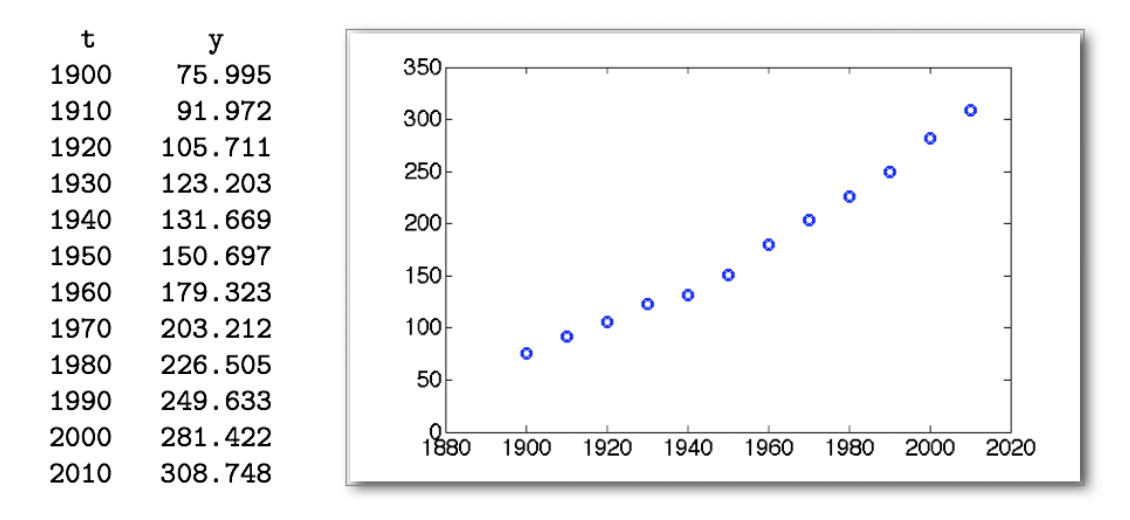
\includegraphics[width=1\linewidth]{images/population.jpg}
\label{fig:population}
\end{figure}

Formulation of least squares (LS) solution:

\begin{description}[font=$\bullet$~\normalfont\scshape\color{red!50!black}]
  \item Polynomial equation 
  \[ y = c_0 + c_1x + c_2x^2 + ... + c_{k-1}x^{k-1} + c_kx^k\]
  \item Given \( m \) points, the system equations can be written as
\begin{figure}[h!]
\centering
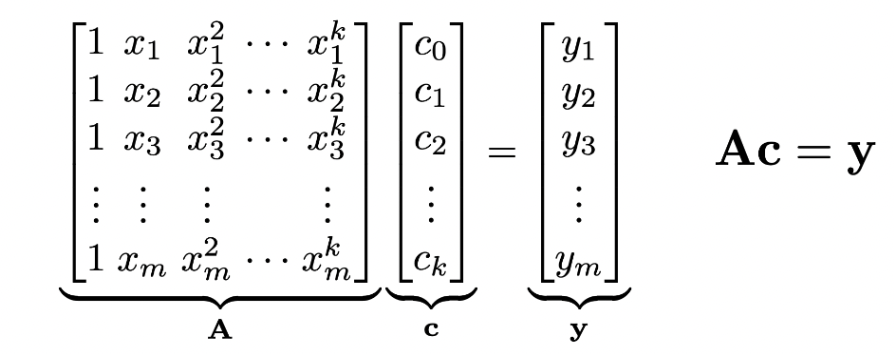
\includegraphics[width=1\linewidth]{images/equation.jpg}
\label{fig:equation}
\end{figure}
  \item Normal equation: \( (\mathrm{A}^\mathrm{T}\mathrm{A})c = \mathrm{A}^\mathrm{T}y\)
  \item LS solution: \( c = (\mathrm{A}^\mathrm{T}\mathrm{A})^{-1}\mathrm{A}^\mathrm{T}y\)
\end{description}

\textbf{Linear line model}

Polynomial equation 
\[ y = c_0 + c_1t \]

The system equations 

\[\begin{bmatrix}
1 & 1900\\
1 & 1910\\
1 & 1920\\
1 & 1930\\
1 & 1940\\
1 & 1950\\
1 & 1960\\
1 & 1970\\
1 & 1980\\
1 & 1990\\
1 & 2000\\
1 & 2010
\end{bmatrix}
\begin{bmatrix}
c_0 \\
c_1
\end{bmatrix} = 
\begin{bmatrix}
75.995\\
91.972\\
105.711\\
123.203\\
131.669\\
150.697\\
179.323\\
203.212\\
226.505\\
249.633\\
281.422\\
308.748
\end{bmatrix}\]

LS solution

\[ c = (\mathrm{A}^\mathrm{T}\mathrm{A})^{-1}\mathrm{A}^\mathrm{T}t = 
\begin{bmatrix}
-3946.3 \\
2.1
\end{bmatrix}\] 

Predict the population for 2020

\[ y = \begin{bmatrix}
1 & 2020 
\end{bmatrix}\begin{bmatrix}
-3946.3 \\
2.1
\end{bmatrix} = 314.4443\]

\begin{figure}[h!]
\centering
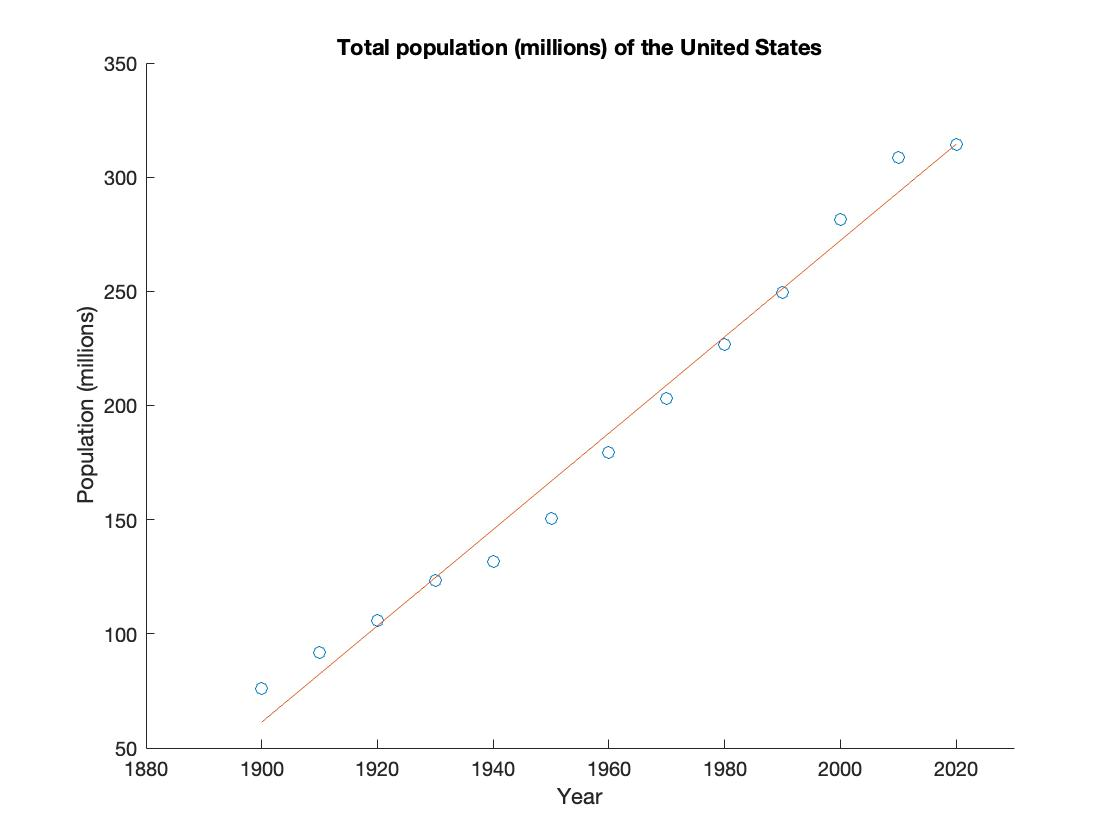
\includegraphics[width=0.6\linewidth]{images/img1.jpg}
\label{fig:img1}
\end{figure}

\textbf{Quadratic parabola model}

Polynomial equation 
\[ y = c_0 + c_1t  + c_2t^2\]

The system equations 

\[\begin{bmatrix}
1 & 1900 & 3610000\\
1 & 1910 & 3648100\\
1 & 1920 & 3686400\\
1 & 1930 & 3724900\\
1 & 1940 & 3763600\\
1 & 1950 & 3802500\\
1 & 1960 & 3841600\\
1 & 1970 & 3880900\\
1 & 1980 & 3920400\\
1 & 1990 & 3960100\\
1 & 2000 & 4000000\\
1 & 2010 & 4040100
\end{bmatrix}
\begin{bmatrix}
c_0 \\
c_1 \\
c_2
\end{bmatrix} = 
\begin{bmatrix}
75.995\\
91.972\\
105.711\\
123.203\\
131.669\\
150.697\\
179.323\\
203.212\\
226.505\\
249.633\\
281.422\\
308.748
\end{bmatrix}\]

LS solution

\[ c = (\mathrm{A}^\mathrm{T}\mathrm{A})^{-1}\mathrm{A}^\mathrm{T}t = 
\begin{bmatrix}
30825 \\
-33 \\
0.0091
\end{bmatrix}\] 

Predict the population for 2020

\[ y = \begin{bmatrix}
1 & 2020 & 2020^2
\end{bmatrix}\begin{bmatrix}
30825 \\
-33 \\
0.0091
\end{bmatrix} = 342.0486\]

\begin{figure}[h!]
\centering
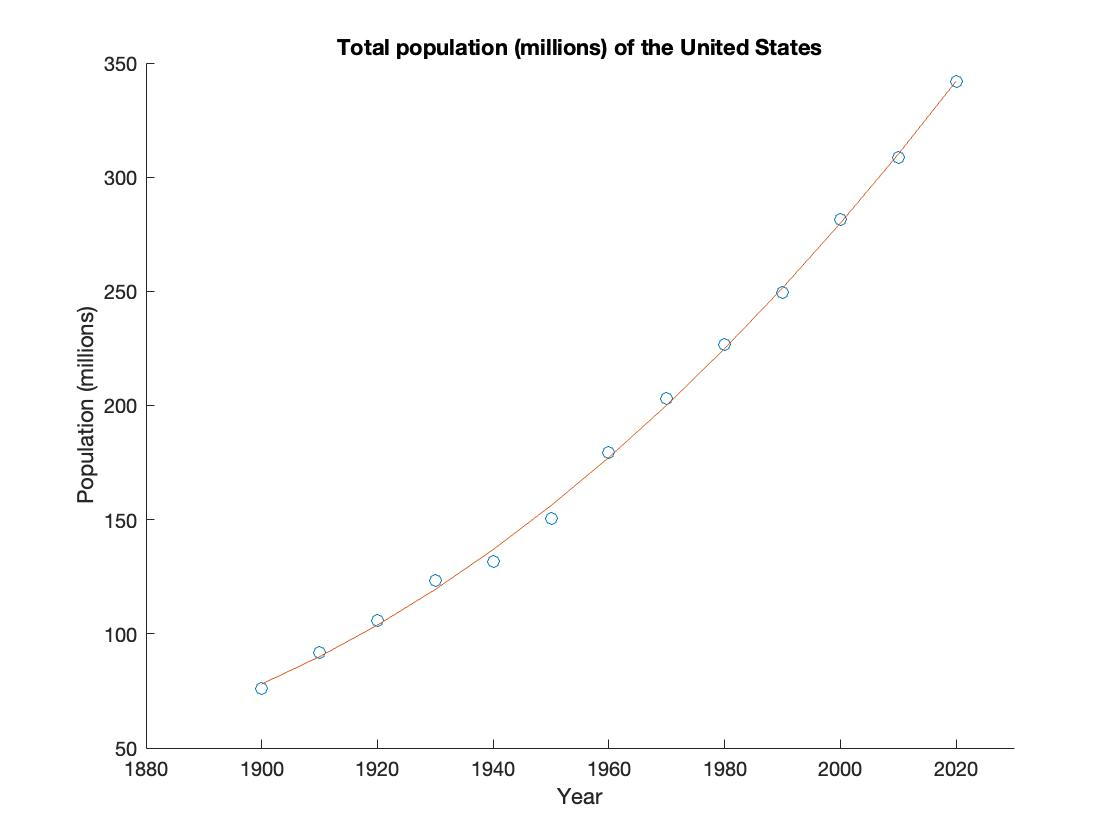
\includegraphics[width=0.6\linewidth]{images/img2.jpg}
\label{fig:img2}
\end{figure}
 
\clearpage
\section{Part 2}
\subsection{Brief Description of MLESAC Algorithm}

Maximum Likelihood Estimator Sample Consensus (MLESAC) is a new robust estimator which is a generalization of the Random Sample Consensus (RANSAC) algorithm. The same sampling approach is used to create putative solutions, but instead of focusing just on the number of inliers, the solution is chosen to maximise likelihood. Using the results of MLESAC, the algorithm's second component provides a general-purpose technique for automatically parametrizing these relations.

The RANSAC algorithm has demonstrated great success in robust estimating, but it is clear that RANSAC can be improved once the robust negative log likelihood function \( -L \) is chosen as the quantity to be reduced.

\begin{multline*}
-L = -\sum_{i} log(\gamma(\frac{1}{\sqrt{2\pi}\sigma})^n
\exp(-(\sum_{j=1,2} {(\underline{x}_i^j - x_i^j)^2 + \\ 
(\underline{y}_i^j - y_i^j)^2})/(2{\sigma}^2) + (1-\gamma)\frac{1}{v}))
\end{multline*}

It makes logical to use this as the score for each of the random samples as the goal is to minimise the negative log likelihood of the mixture \( -L \). The issue is that the mixing parameter \( \gamma \) cannot be seen directly. However, since this is a one-dimensional search, there is no processing overhead, and it is easy to retrieve \( \gamma \) that yields the smallest \( -L \) given any putative solution for the model's parameters.

To estimate \( \gamma \), using Expectation Maximization (EM), a set of indicator variables needs to be introduced: \( \eta_i, n = 1...n \), where \( \eta_i = 1 \) if \( i \)th correspondence is an inlier, and \( \eta_i = 0 \) if \( i \)th correspondence is an outlier. The EM algorithm proceeds as follows treating the \( \eta_i \) as missing data: 

\begin{enumerate}
  \item Generate a guess for \( \gamma \).
  \item Estimate the expectation of the \( \eta_i \) from the current estimate of \( \gamma \).
  \item make a new estimate of \( \gamma \) from the current estimate of \( \eta_i \) and go to step (2).
\end{enumerate}

This approach is known as MLESAC (maximum likelihood consensus). Putting a prior on \( \gamma \), the expected proportion of inliers, is occasionally useful for real systems; however, this is not followed further here because it depends on the application. An initial estimate of the relation and the likelihood that each correspondence is consistent with the relation are the outputs of MLESAC, similar to RANSAC. The estimation of the relation is then improved using the gradient descent method.

On both real and fake data, the various parametrizations were tested in the study. Two metrics are contrasted: The accuracy of the solution is evaluated in the first. The second metric is the quantity of cost function evaluations, or how frequently \( D \) is assessed. When dealing with artificial data, the initial step is

\[ \sigma_p = (\sum_{ij} \frac{d^2(\hat{x}_i^j,\underline{x}_i^j)}{n})^\frac{1}{2} \]

for the set of inliers, where \( \hat{x}_i^j \) is the point closest to the noise free datum  \( \underline{x}_i^j \) which satisfies the image relation, \( x_i^j \) is the point \( i \)th in the \( j \) image, and The Euclidean distance between the points is denoted by the symbol \( d() \). This gives an indication of how far the estimated connection is off from the actual data; in other words, we compare the fit of our calculated relation derived from the noisy data against the established ground truth. The standard deviation of the inliers is used to evaluate the accuracy of real-world data

\[ \sigma_r = (\sum_{i} \frac{e_i^2}{n})^\frac{1}{2} \]

Stage 2's initial estimation of the seven-point basis for basic matrices or crucial surfaces, or the four-point basis for image-image homography or projectivity, is relatively near to the actual solution, hence stage 3 often avoids local minima. In general, much more function evaluations are needed during the non-linear minimization step than during the random sampling phase. The number necessary, which varies with parametrization, serves as a second criterion (in addition to variance) for evaluating the parametrization.

When the data are tainted by outliers, it has been found that the MLESAC approach of robust fitting works well for initialising the parameter estimation. In this instance, a data can only belong to one of the two classes—inliers or outliers. The MLESAC approach can be extended to situations where the data came from a more extensive mixture model with several classes, including clustering issues.

An enhancement over RANSAC in this study research: MLESAC has proven to provide more accurate estimations. It has been proven that an universal method for constrained parameter estimate produces results that are on par with or better than those of the methods now in use. To estimate and parametrize complicated quantities like critical surfaces, there aren't many general-purpose methods available. Other estimate issues in vision, such as estimating the Quadrifocal tensor between four images, complex polynomial curves, etc., could be solved using the generic method (of minimal parametrization in terms of basis points found via MLESAC). Any problem where basic parametrizations are not immediately apparent and the relations may be discovered from a small number of points could be solved using the general methods outside of vision.

\clearpage

\subsection{Sphere Fitting from 3D Point Cloud}

\begin{lstlisting}[language=Matlab]

% Assignment 3
% Part 2

% Load a point cloud into the workspace
load("object3d.mat");

% Display the point cloud 
% and label the figure
figure
pcshow(ptCloud)
xlabel("X(m)")
ylabel("Y(m)")
zlabel("Z(m)")

\end{lstlisting}

\begin{figure}[h!]
\centering
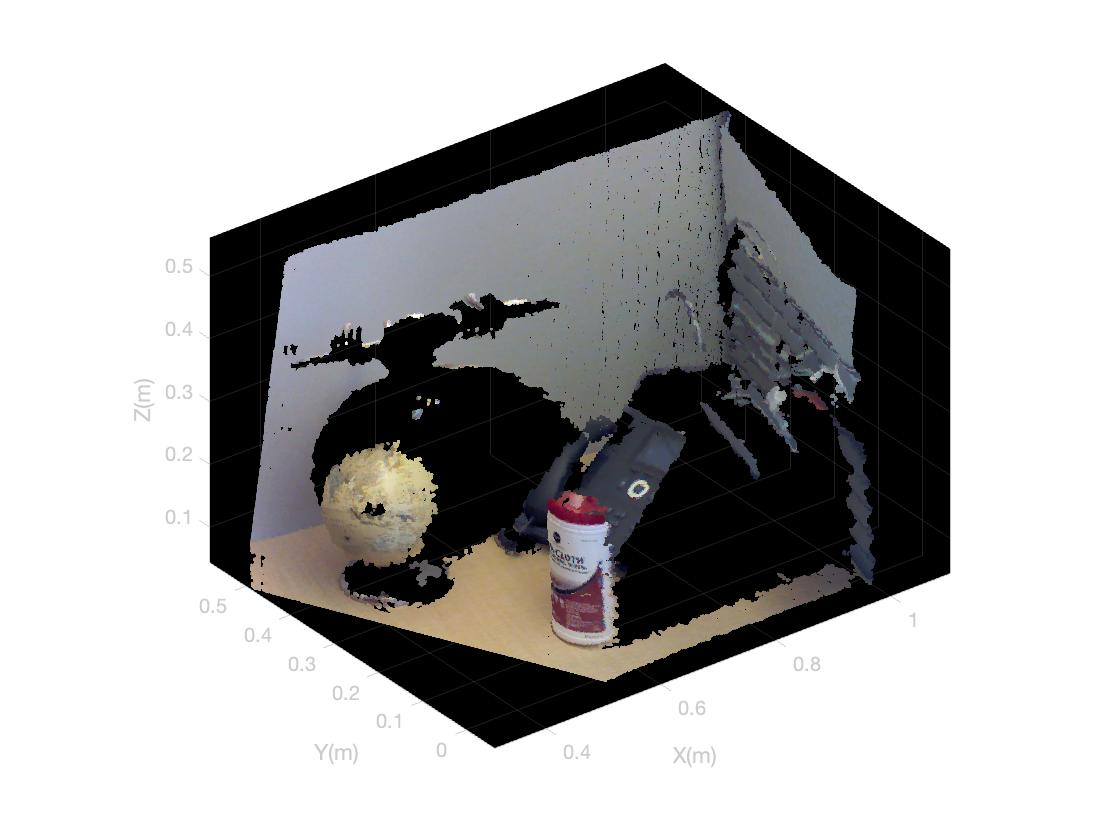
\includegraphics[width=0.8\linewidth]{images/object.jpg}
\caption{Detect a sphere in a point cloud}
\label{fig:object}
\end{figure}

\begin{lstlisting}[language=Matlab]

% Set the maximum point-to-sphere 
% distance for sphere fitting to 1cm
maxDistance = 0.01;

% Set the region of interest to 
% constrain the search
roi = [0.3,0.5;0.2,0.4;0.1,0.4];
sampleIndices = findPointsInROI
(ptCloud,roi);

% Detect the globe in the 
% point cloud and extract it
[model,inlierIndices]=pcfitsphere(ptCloud,
maxDistance,SampleIndices=sampleIndices);
globe = select(ptCloud,inlierIndices);

% Plot the extracted globe
figure
pcshow(globe)

\end{lstlisting}

\begin{figure}[H]
\centering
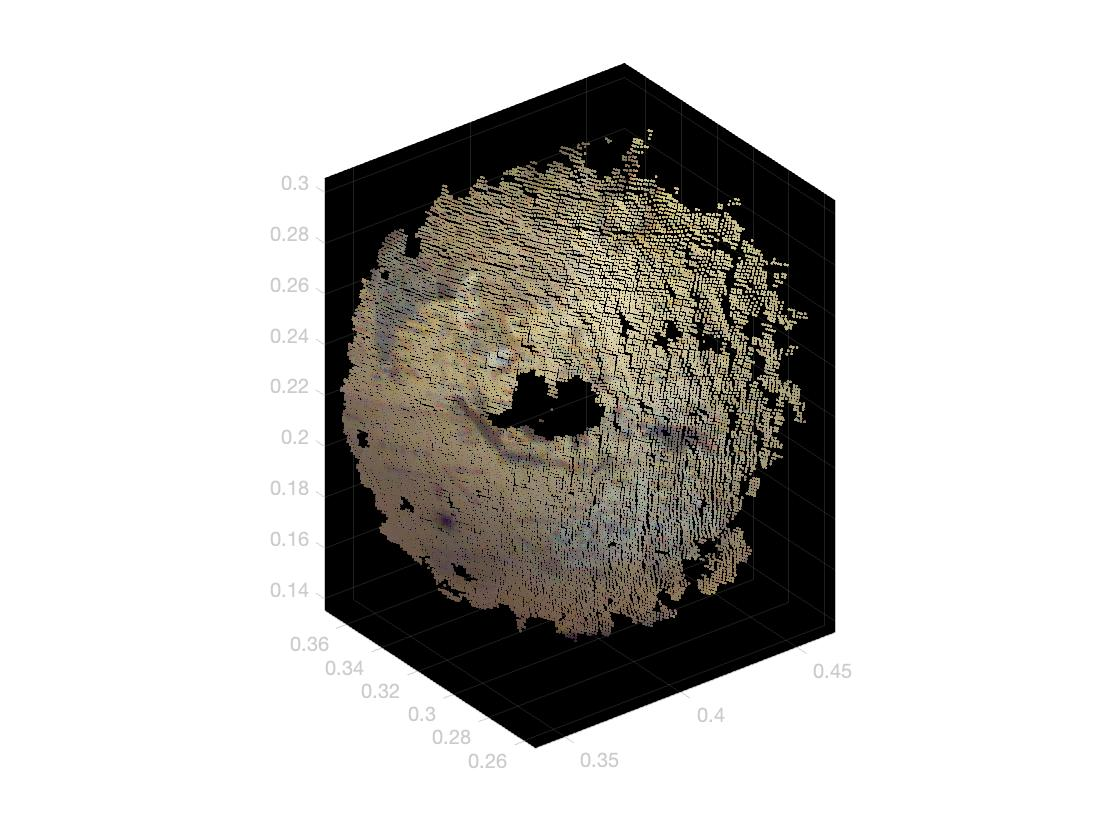
\includegraphics[width=0.8\linewidth]{images/globe.jpg}
\caption{Globe Point Cloud}
\label{fig:globe}
\end{figure}

\clearpage

\section{Part 3}

As mentioned in previous assignment, the topic to be worked on is handwritting recognition. The objective of this project is to create a machine learning model that is able to identify any handwritten letters or digits. The approach to this problem is to use deep learning since it is known as a high-accurate method for recognition. Currently, the process is starting with in-depth researches about the intuition behind Artificial Neural Networks (ANN), Convolutional Neural Networks (CNN), and Recurrent Neural Networks (RNN) and how to apply them to the problem. Additionally, one of the most important task is to collect a good labelled dataset for training and testing ML model. 

For group enrollment, I joined in Group 5 with other two students.

\end{document}
